\documentclass[aspectratio=169]{beamer}
\usetheme{Madrid}
\usecolortheme{default}

\usepackage{graphicx}
\usepackage{tikz}
\usepackage{amsmath}
\usepackage{hyperref}
\usepackage{animate}

\title{Process Mining: From Theory to Practice}
\subtitle{A Lightning Introduction}
\author{Garrett Gruss}
\institute{CS8317 Sect 795A 1262}
\date{\today}

\begin{document}

% Slide 1: Title
\begin{frame}
\titlepage
\end{frame}

% Slide 2: What is Process Mining?
\begin{frame}{What is Process Mining?}
\begin{itemize}
    \item \textbf{Bridge between data science and process management}
    \item Discovers graphs from event log data
    \item Discover relationships between actors within event data
    \item Monitor event logs for deviations from graph
\end{itemize}

\vspace{1em}
\begin{center}
\textit{``Process mining is the missing link between model-based process analysis and data-oriented analysis techniques.''}
\end{center}
\end{frame}

% Slide 3: The Pioneer - Wil van der Aalst
\begin{frame}{The Pioneer: Wil van der Aalst}
\begin{columns}
\begin{column}{0.5\textwidth}
% Uncomment and add path to van der Aalst's photo:
\begin{center}
\includegraphics[width=0.7\textwidth]{Wil-van-der-Aalst-177138299.png}
\end{center}
\end{column}
\begin{column}{0.5\textwidth}
    \textbf{Origins \& Background:}
    \begin{itemize}
        \item Eindhoven University of Technology (Netherlands)
        \item Founded process mining discipline in late 1990s/early 2000s
        \item Created PM4PY and ProM frameworks
    \end{itemize}
\textbf{Key Insight:}
\begin{itemize}
    \item Organizations collect massive event logs
    \item Traditional analysis misses hidden patterns
    \item Automated discovery reveals actual workflows
\end{itemize}
\end{column}
\end{columns}
\end{frame}

% Slide 4: Van der Aalst's Original Motivation
\begin{frame}{Original Motivation: Understanding Reality vs. Models}
\textbf{The Problem:}
\begin{itemize}
    \item Process models often outdated or idealized
    \item Gap between ``how we think it works'' vs. ``how it actually works''
    \item Manual analysis too time-consuming and error-prone
    \item \textit{Example:} Engineers manually tracing telemetry after failures
\end{itemize}

\vspace{1em}
\textbf{The Vision:}
\begin{itemize}
    \item \textbf{Process Discovery:} Automatically extract models from event logs
    \item \textbf{Conformance Checking:} Compare reality vs. intended process
    \item \textbf{Enhancement:} Identify bottlenecks and predict failures
\end{itemize}

\vspace{0.5em}
\textit{\small Originally business processes, now applicable to any event-driven system}
\end{frame}

% Slide 5: Process Discovery - The Alpha Miner
\begin{frame}{Process Discovery: The Alpha Miner Algorithm}
\textbf{How It Works:}
\begin{itemize}
    \item Van der Aalst's foundational algorithm (2004)
    \item Analyzes \textbf{temporal ordering} of activities in event traces
    \item Constructs Directly-Follows Graph (DFG) by correlating events
\end{itemize}

\vspace{1em}
\textbf{Event Trace Example:}
\begin{center}
\small
Case 1: \texttt{[Created → Assigned → Started → Resolved → Closed]}\\
Case 2: \texttt{[Created → Assigned → Started → Escalated → Resolved → Closed]}
\end{center}

\vspace{1em}
\textbf{The Algorithm Identifies:}
\begin{itemize}
    \item \textbf{Direct succession:} If activity B follows A, create edge A → B
    \item \textbf{Parallelism:} Activities that occur in any order
    \item \textbf{Choice:} Alternative paths (escalated vs. direct resolution)
    \item \textbf{Transition counts:} Frequency of each path
\end{itemize}
\end{frame}

% Slide 6: Demo Overview
\begin{frame}{Demo: IT Ticket Process Mining}
\textbf{Use Case:} Converting semi-structured events into a system process diagram

\vspace{1em}
\textbf{Dataset:}
\begin{itemize}
    \item Synthetic IT helpdesk tickets
    \item Multiple departments (Finance, Engineering, HR, Operations, Sales)
    \item Various categories (Software, Hardware, Network, Access, Security)
    \item 52 tickets with complete lifecycle events
\end{itemize}

\vspace{1em}
\textbf{Tools:}
\begin{itemize}
    \item PM4PY (Python process mining library)
    \item Pandas for data manipulation
\end{itemize}

\vspace{0.5em}
\textit{\small This demo validates methodology for vehicle telemetry failure detection}
\end{frame}

% Slide 7: Demo Workflow
\begin{frame}{Demo Workflow}
\begin{enumerate}
    \item \textbf{Data Preparation}
    \begin{itemize}
        \item Parse CSV logs into PM4PY event log format
        \item Map: case\_id (ticket\_id), activity, timestamp
    \end{itemize}

    \item \textbf{Process Discovery}
    \begin{itemize}
        \item Generate Directly-Follows Graph (DFG)
        \item Performance DFG with time annotations
        \item Markov chain visualization of variant flows
    \end{itemize}

    \item \textbf{Variant Analysis}
    \begin{itemize}
        \item Identify nominal vs. alternate paths
        \item 20 unique process variants discovered
        \item Top variant: 28.85\% (standard resolution path)
    \end{itemize}
\end{enumerate}
\end{frame}

% Slide 8: Process Visualizations
\begin{frame}{Process Visualizations}
    \begin{columns}
    \begin{column}{0.5\textwidth}
        \includegraphics[width=0.8\textwidth]{example_3_dfg_markov.png}
        \small{Directly-Follows Graph showing transition probabilities between ticket states}
    \end{column}
    \begin{column}{0.5\textwidth}
        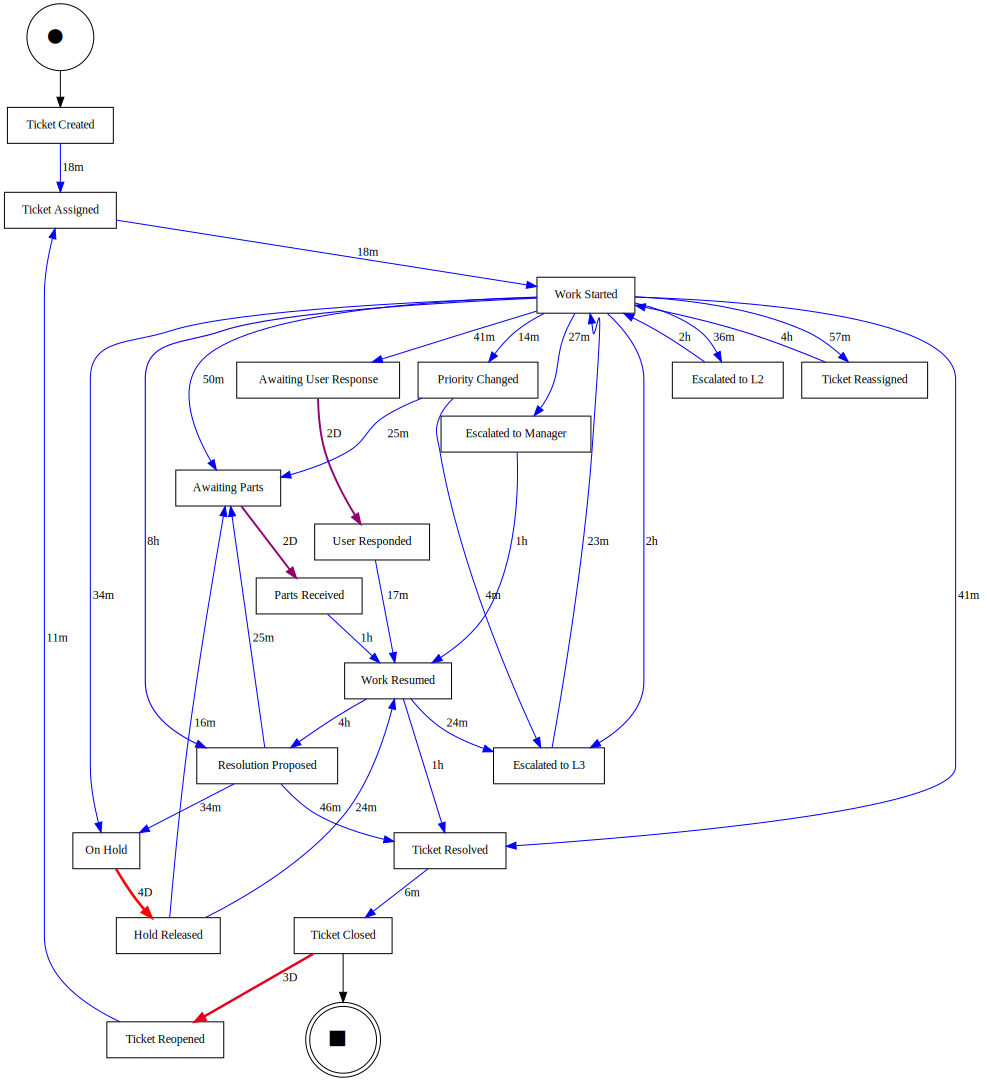
\includegraphics[width=0.8\textwidth]{example_3_dfg_performance.png}
        \small{Performance DFG with average timing between events (in seconds)}
    \end{column}
    \end{columns}
\begin{center}
\end{center}
\end{frame}

% Slide 10: Key Discoveries
\begin{frame}{Key Discoveries from the Analysis}
\textbf{Process Variants:}
\begin{itemize}
    \item \textbf{Happy Path (28.85\%):} Created → Assigned → Started → Resolved → Closed
    \item \textbf{User Interaction (11.54\%):} Includes ``Awaiting User Response'' cycle
    \item \textbf{Escalation Path (11.54\%):} L2 escalation with additional work
\end{itemize}

\vspace{1em}
\textbf{Performance Metrics:}
\begin{itemize}
    \item Average wasted time: \textbf{10.81 hours per ticket}
    \item Flow rate (efficiency): \textbf{1.92\%}
    \item High priority tickets: 55.6k seconds avg wasted time
\end{itemize}
\end{frame}

% Slide 11: Organizational Insights
\begin{frame}{Organizational Role Discovery}
\textbf{Technician Performance Analysis:}
\begin{itemize}
    \item \textbf{Most Efficient:} Sam Williams (5,023s avg wasted time)
    \item \textbf{Highest Workload:} Alex Martinez (59,326s avg wasted time)
    \item Discovered role-based patterns using PM4PY organizational mining
\end{itemize}

\vspace{1em}
\textbf{Category-Based Insights:}
\begin{itemize}
    \item Security tickets: Most efficient (16,702s avg)
    \item Hardware tickets: Longest delays (55,386s avg)
    \item Software tickets: Highest variety (16 tickets)
\end{itemize}
\end{frame}

\end{document}
